\documentclass[10pt,conference]{IEEEtran}
%\documentclass[letterpaper,twocolumn,10pt]{article}

\usepackage{graphicx}
\usepackage{url}
\usepackage[usenames]{color}
\usepackage{listings}
\usepackage{wrapfig}
\usepackage[caption=false]{subfig}


%------------------------------------------------------------------------- 
% take the % away on next line to produce the final camera-ready version 
\pagestyle{empty}

%------------------------------------------------------------------------- 
\begin{document}

\title{Continuous Integration of Software Management}


%for single author (just remove % characters)
\author{
{\rm Gautam Kumar, Prof. David Socha}\\
Computing and Software Systems\\
University of Washington Bothell\\
gautamk@uw.edu, socha@uw.edu
} % end author

\maketitle
\thispagestyle{empty}


\section*{Abstract}
Continuous Integration, A practice where developers integrate 
frequently\cite{stahl_modeling_2014} is considered an integral part of Agile 
development. CI is often thought to be a safety net that prevents developers from deploying broken code to production. 

A similar process and ideology of continual improvement and integration can be applied to Software Management, The art and science of planning and leading software projects \cite{stellman_applied_2005}.

This paper attempts to explore the process of creating such an integration practice within an Organisation.

\subsubsection*{Keywords}

Software Management, Agile development, Continuous Integration

\section*{Introduction}

Martin Fowler in his seminal article\cite{fowler_continuous_2006} on Continuous Integration describes it as a practice where members of a team integrate their work frequently and each integration is verified by an automated build to detect problems quickly.

In the context described above integration is the process of combining the work of all the developers of a project into a cohesive software. On the other hand if considered generically, Integration can be thought of as a practice of combining the work of multiple people and verifying its correctness. Using a similar collective, Continuous integration could be the process if integrating the work of multiple people after specific events or set periods of time. 

\section*{Continuous Improvement}

The practice of continuous improvement has evolved as a response to improvements in the way software is delivered and used by customers. With the introduction and popularisation of the internet in the early years of the 21st century many consumers and enterprises started using the internet and web technologies as more than just an information directory. Web sites evolved into web apps which lead to the rise of Web 2.0 \cite{oreilly_what_2007}. This evolution to Web 2.0 required innovations with web server technologies which also introduced significant complexity and risk to the stability of the software systems \cite{oreilly_what_2007}.

Continuous Integration evolved in response to the increased risk to software stability and attempts to act as a safety net \cite{fowler_continuous_2006} to developers. Continuous Integration doesn't actually prevent or fix bugs, it merely makes discovering bugs easier and faster. 

\section*{Software Management and Continuous Improvement}

The inherent complexity in software management is best described by the law of leaky abstractions\cite{spolsky_law_2002} which states that all non-trivial abstractions leak to some degree. 

Software management is in essence a process which tries to abstract away the chaos of managing an inherently complex task with the help of developers in an ever-evolving environment. So naturally Software Management tends to be a complex task which needs to be continually improved to adapt to changes in the environment such as new labour laws, new technologies and a new generation of customers and	 developers. 

\section*{CI and an Evolving Environment}

\subsection*{Evolving Customer}
The previous generation of customers were primarily using a desktop computer with a reliable internet connection and a large display. This customer base is quickly moving towards mobile devices as their primary computing device where displays are much smaller, internet connection is spotty and there are restrictions on power consumption. 

These changes require the developers to adapt to the environment which inherently needs an overhaul of the software management process. 


\subsection*{TODO: New technologies}
\subsection*{TODO: Labour laws}
\subsection*{TODO: Next Gen Developers}

\section*{Implementing CI in Software Management}

Continuous Integration and Improvement by nature is an iterative process thus implementing within the context of Software management requires the management team to follow a disciplined process of continuous evaluation and an evolution.

\subsection*{Adoption}
The initial adoption process of any new Software management model would be significantly different from integrating new team members into an existing model. For example, some the factors which affect the success of adopting Agile methodologies in an organisation are 
Customer collaboration, satisfaction and commitment, Communication and negotiation skills of the team and Cultural factors \cite{misra_identifying_2009}.

These success factors differ when brining in new team members. For example a team member fresh out of college might adapt to an existing process at an organisation with ease while a seasoned developer who is loyal to the waterfall model might have a hard time adapting to the rapid pace of an agile organisation. 

As teams being to understand the expectations of their customers and their organisations the previously defined software process evolves thus as time goes on each team / organisation starts building a unique variation of the agile process.

In this context initial adoption is usually the easiest task as the whole team is collectively working towards making sure that Agile adoption succeeds. Adoption by new team members on the other hand depends on the new team member, the Software management team and the culture of the organisation.

It is the responsibility of the software management team to enable new developers to adopt and adapt to the unique process of the dev team they are going to be working with.

\begin{figure}[t]
\centering
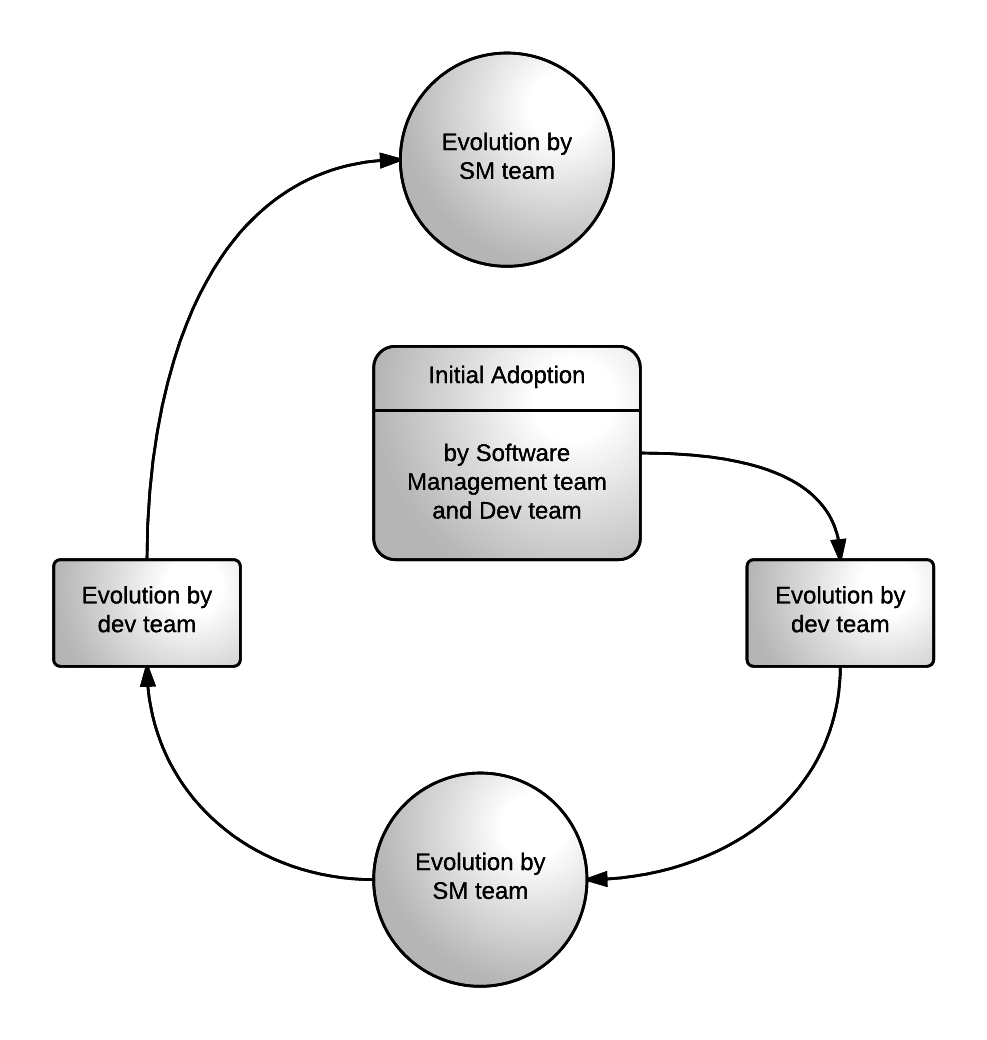
\includegraphics[width=0.5\textwidth]{sm_dev_team_process_evolution.png}
\caption{The Software management team has to evolve the adoption process as the dev team deviates from the initial Software developement model}
\end{figure}

\subsubsection*{Success criteria} The software management team needs to have a clear and evolving success criteria which monitors the each new hire and how well they are able to adapt to their new teams. This differs from Definition of Done (DoD) based on the fact that DoD is merely a set of activities which need to be performed to get the user story to a shippable state while Success criteria is a broader set of expectations from the candidate which are recorded based on subjective observations. 






\bibliographystyle{plain}
\bibliography{css566_software_management}

\end{document}

